We designed the frontend, called as Memmetric, in two aspects: \textbf{real-time monitor} and \textbf{historical monitor}. Real-time monitor  presents users the current status of the clusters. Historical monitor records anomalous data points to hint users debug their cluster.

\begin{figure}[h!]
  \caption{Real-time Monitor}
  \centering
    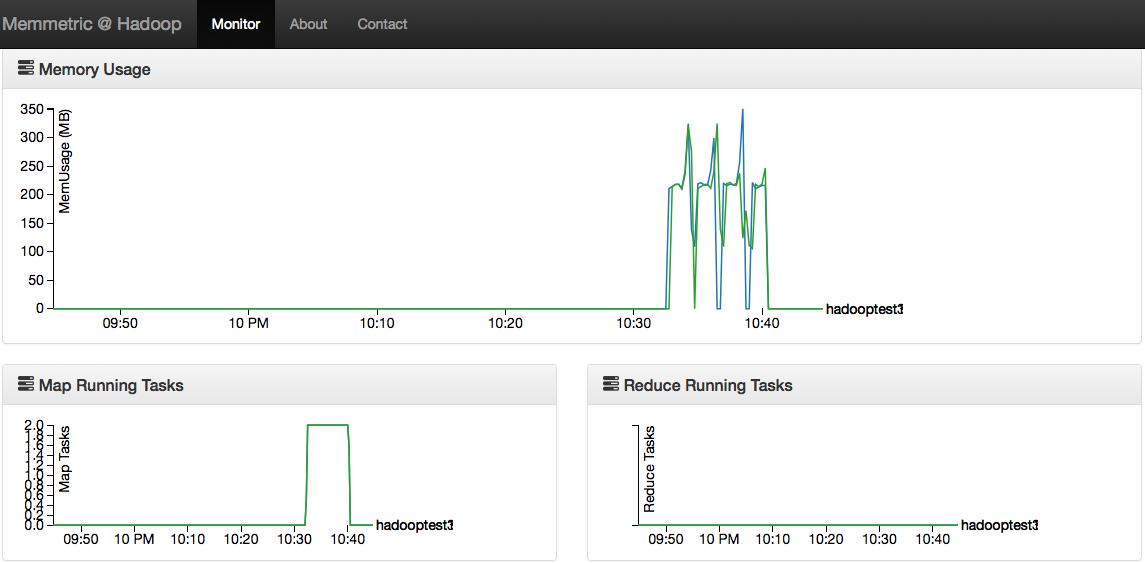
\includegraphics[width=0.5\textwidth]{image/real-time-monitor.png}
\end{figure}

Real-time monitor shows per-machine view of task heap memory usage, the number of running map tasks and reduce tasks. Each line in "Memory Usage" block shows the total heap memory usage in a machine. Also, lines in "Map Running Tasks" and "Reduce Running Tasks" show the number of map an reduce tasks in different machines.

Hadoop cluster reports the memory usage for each task to Ganglia. However, plotting the memory usage of all tasks individually on the same chart can be hard to understand, because a Hadoop job may spawn hundreds of tasks. Therefore, Memmetric aggregates all per-task heap memory usage on a machine into a per-machine heap memory usage line. Also, Memmetric shows the number of running map tasks and reduce tasks. Real-time monitor provides a clue whether there are tasks killed due to over memory usage. If there is a sharp drop of heap memory usage on machine, it is possible that some tasks use too many memory to be killed by JVM or operating system. 

\begin{figure}[h!]
  \caption{Historical Monitor and Parameter Settings}
  \centering
    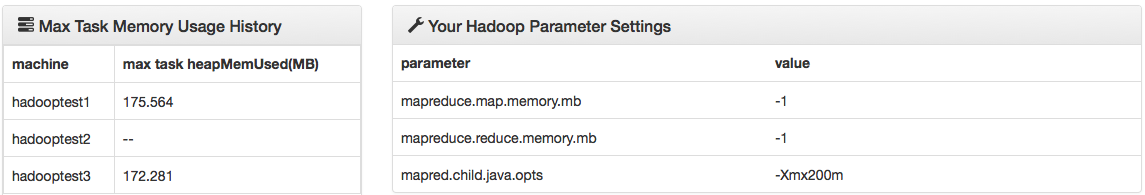
\includegraphics[width=0.5\textwidth]{image/historical-monitor.png}
\end{figure}

Historical monitor presents the odd data points in each machine for users to revise their cluster parameter settings. Memmetric records the data points of largest task heap memory usage in each machine, because those points are the possible moments where a task violates the memory upper bound restriction and results in failure. For example, if Hadoop cluster sets "mapred.child.java.opt" as "-Xmx200m", which means that  the JVM child of a task at most allocate 200MB memory. If the historical monitor shows that some task has used more than 200MB, it is highly possible that the task will be killed, and the user should consider to modify the parameter to enlarge the maximum heap memory usage.

\begin{figure}[h!]
  \caption{Memmetric Overview}
  \centering
    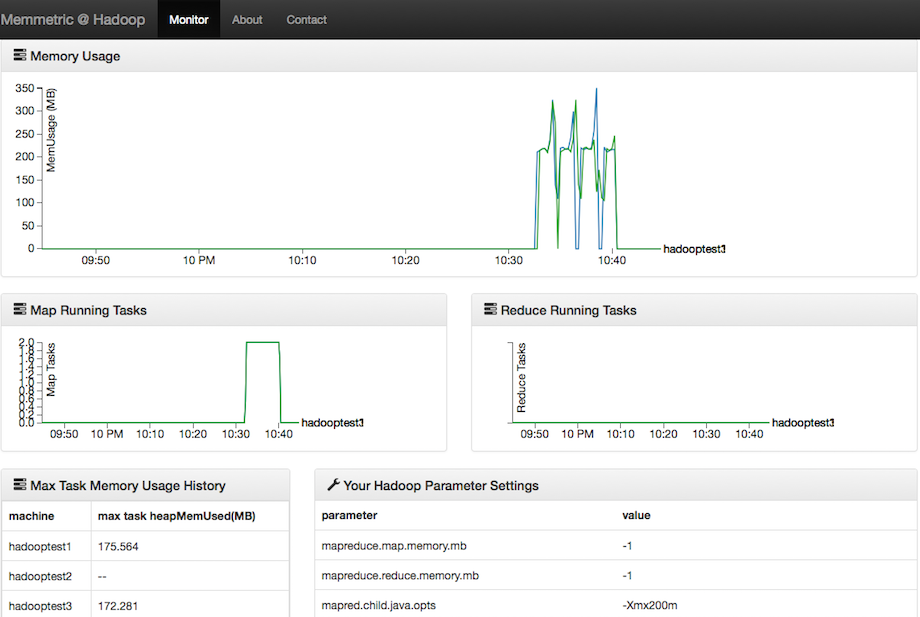
\includegraphics[width=0.5\textwidth]{image/overview.png}
\end{figure}